\chapter{Johannes Work}
\section{BLOB-Analysis}
A common problem when dealing with images is to determine if the image data contains a particular object or shape. The term BLOB stands for Binary Large Objects and refers to a region of connected pixels in a binary image. This technique is used to extract meaningful information from images, separate the pixels by detecting the points or regions that differ in properties like brightness or color changes (i.e., their value), and classify them into two categories: the foreground (pixels with a non-zero value) and the background (pixels with a zero value).
Therefore, BLOB analysis will be split in three main steps: \textit{Extraction} of the BLOBs, \textit{representation} of the BLOBs and lastly, \textit{classification} of the BLOBs to know which ones belong to the expected type.
\subsection{BLOB Extraction}
To isolate BLOBs in a binary image, the first step is to define whether two pixels are connected or not. This is done by applying algorithms that will help to determine the connectivity of the pixels, but also the number of BLOBs contained in an image. The most common used connectivities in BLOB extraction are the 8-connectivity and the 4-connectivity kernels. The 8-connectivity kernel is more accurate than the 4-connectivity kernel, but it also requires more computations and consequently needs more time to process the image.

%% add picture here

\subsubsection{Grass-Fire Algorithm}
One of these connected component labeling algorithm is the \textbf{Recursive Grass-Fire Algorithm}. This algorithm is used to erode images but also to track the pixels locations to create a region.
To explain and visualise this algorithm, a test with both 8-connectivity and 4-connectivity kernels are mare, to give an overview of how these choices can affect the final result. \fixme{How it works should be explained before running the test. There is no explanation of the different directions the kernels can burn, and which ways it prioritise first etc.}

\begin{figure}[htbp]
\centering
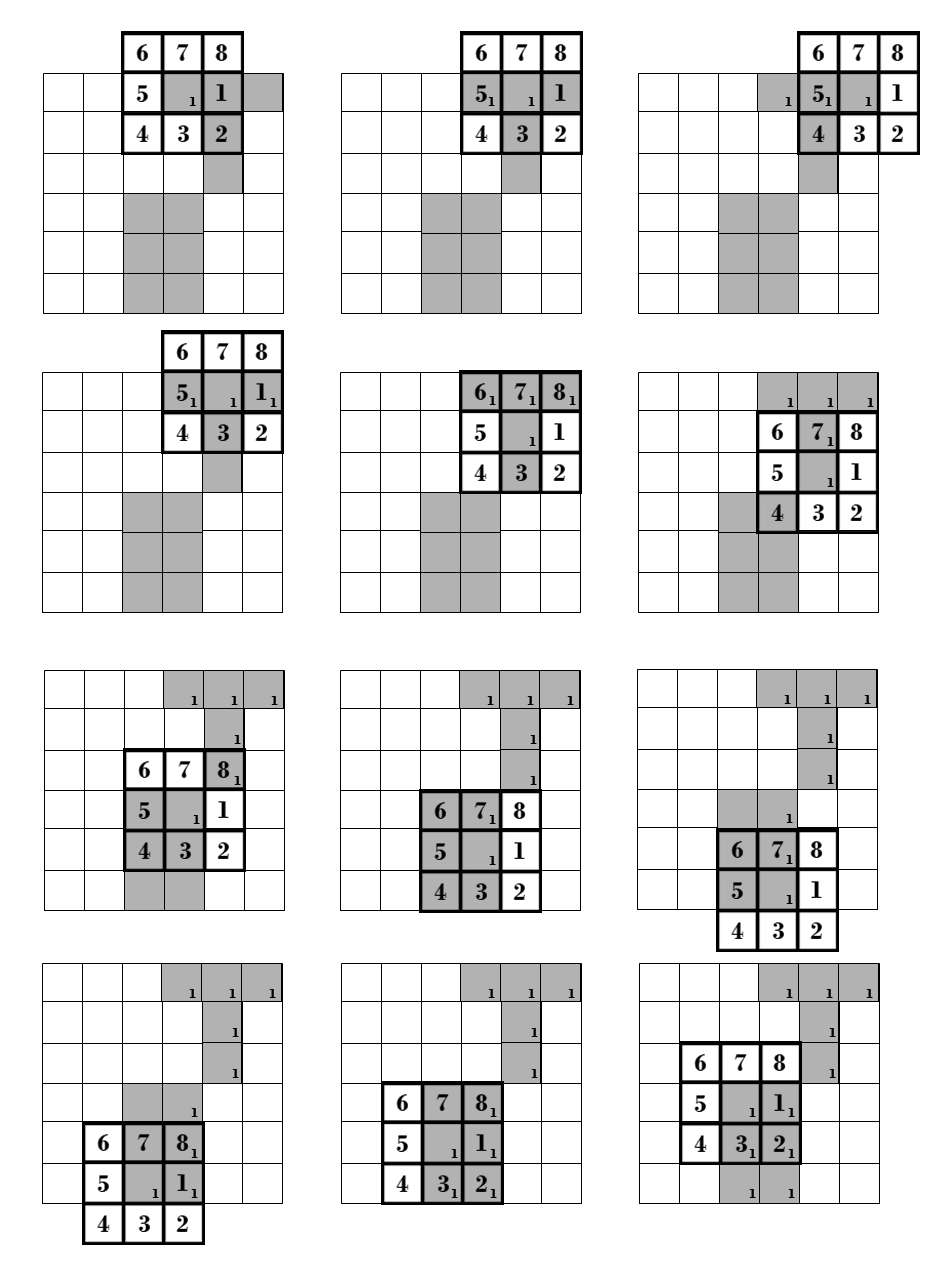
\includegraphics[width=0.8\textwidth]{Pictures/Theory/8connec_kernel.png}
\caption{8 connectivity labeling kernel detects 1 single object}
\label{fig:8connecK}
\end{figure}

As figure \eqref{fig:8connecK} illustrates, the Grass-Fire algorithm scans the whole image from the upper-left side to the right bottom row by row. When the kernel finds a non-zero pixel value it centers its attention on it and burns \fixme{Explain what "burns" means} it. Then the algorithm looks in the possible directions around that pixel to check if one of those pixels is connected to the previous one, and therefore, is an object \fixme{Isn't a single pixel an object as well?}. The way the algorithm will do this will depend on the connectivity used (for a 8-connectivity kernel, the algorithm will look into 8 directions, but for the 4-connectivity kernel, the algorithm will look in just 4 directions).
Whenever it finds an object, the algorithm labels the pixel on the output image and then burns that pixel on the input image in order to turn it into a zero and ensure that the pixel will not be part of a new grassfire.
Now the algorithm looks on the possible directions around that pixel, starting with the pixel on the right (see kernel picture \eqref{fig:8connecK}). Once it finds a non-zero pixel value, the algorithm centers its attention on it and restarts the process again labeling the pixel with the number of the previous one. At the end of that row the algorithm will check the surrounding pixels on the row below. If a non-zero pixel value is found, the algorithm will continue the process of burning and labeling pixels, otherwise the algorithm will starts its way back to the beginning checking one by one surrounding pixels to verify that it has checked all the possible directions and non-zero pixels values.
Comparing the figure \eqref{fig:8connecK} and the figure \eqref{fig:4connecK}, we can realize how the choice of a certain connectivity kernel will affect the final result of the algorithm using a same picture. Although the 8-connectivity kernel is more accurate it seems to be unable to separate the different objects correctly, whereas the 4-connectivity kernel finds the different objects performing less operations.

\begin{figure}[htbp]
\centering
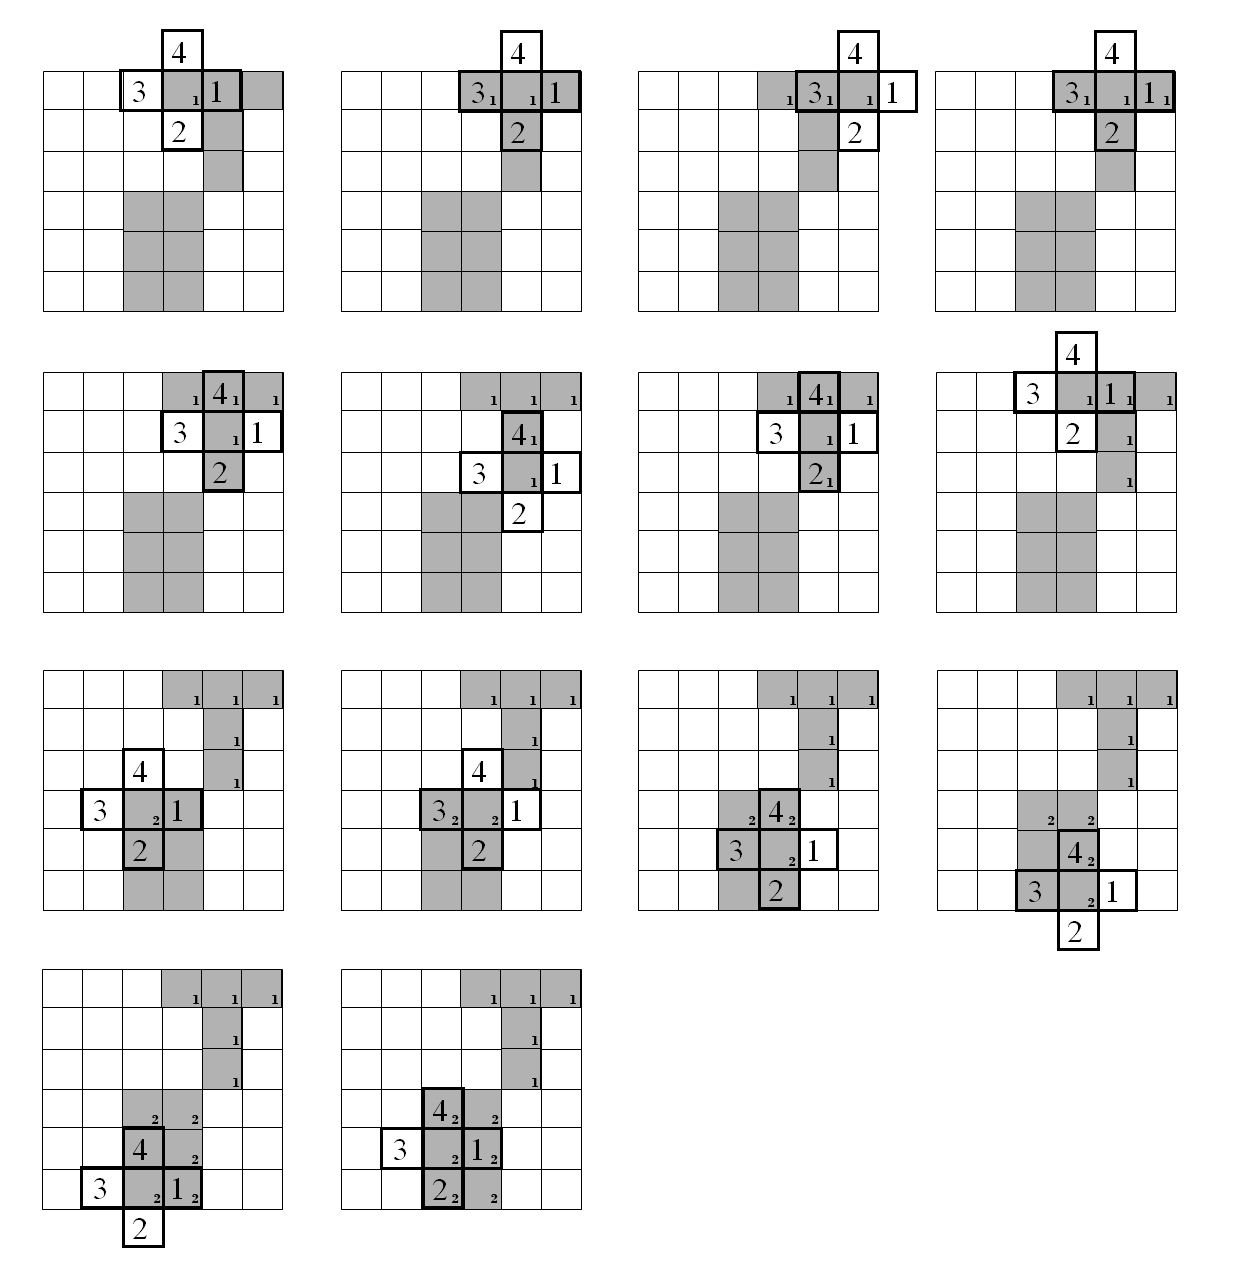
\includegraphics[width=0.75\textwidth]{Pictures/Theory/4connec_kernel.png}
\caption{4 connectivity labeling kernel detects 2 objects}
\label{fig:4connecK}
\end{figure}



Figure \eqref{fig:4connecK}